%% =====================================================================
%%  Robin — Informe Final (Hito 3)
%%  Universidad Mayor · INGT1003-001 · Arquitectura de Desarrollo Móvil y Web
%%  Autores: Lucas Calquín, Nicolás Escobar · Docente: Carlos Muñoz
%%
%%  Compilar con pdfLaTeX (2 pasadas, para índice y fondos TikZ).
%%  Archivos necesarios en la misma carpeta (o en ./img/):
%%      portada.jpg   logo_umayor.png
%%  NOTA (Fase 1): se reutilizó el mismo portada.jpg del Hito 2. Si el título
%%  "Hito 2" está dibujado dentro de esa imagen (no como texto LaTeX), hace
%%  falta una imagen nueva para "Hito 3" — confirmar con el equipo.
%% =====================================================================
\documentclass[11pt,letterpaper]{article}

% ---------------------------------------------------------------- Codificación e idioma
\usepackage[utf8]{inputenc}
\usepackage[T1]{fontenc}
\IfFileExists{spanish.ldf}{%
  \usepackage[spanish,es-noshorthands]{babel}%
}{%
  % Respaldo si babel-spanish no está instalado: sin silabeo (evita cortes erróneos)
  \hyphenpenalty=10000 \exhyphenpenalty=10000
}
\DeclareUnicodeCharacter{2192}{\ensuremath{\rightarrow}}
\DeclareUnicodeCharacter{2014}{---}

% ---------------------------------------------------------------- Tipografía (equivalente a Arial)
\usepackage{helvet}
\renewcommand{\familydefault}{\sfdefault}
\usepackage{courier}
\usepackage{microtype}
\usepackage{setspace}
\linespread{1.18}\selectfont
\setlength{\parindent}{0pt}
\setlength{\parskip}{6pt plus 1pt}
\emergencystretch=3em

% ---------------------------------------------------------------- Página
\usepackage[letterpaper,left=1.2in,right=1.2in,top=1.55in,bottom=1.1in,
            headheight=18pt,headsep=0.2in,footskip=0.42in]{geometry}

% ---------------------------------------------------------------- Colores corporativos
\usepackage[table,dvipsnames]{xcolor}
\definecolor{mayorgreen}{RGB}{56,118,29}
\definecolor{mayordark}{RGB}{39,78,19}
\definecolor{robingreen}{RGB}{71,110,73}
\definecolor{robinorange}{RGB}{221,110,17}
\definecolor{cream}{RGB}{245,244,237}
\definecolor{softgreen}{RGB}{234,242,228}
\definecolor{lightgreen}{RGB}{183,206,174}
\definecolor{codebg}{RGB}{13,17,23}
\definecolor{codefg}{RGB}{201,209,217}
\definecolor{jsgreen}{RGB}{138,214,120}
\definecolor{jsblue}{RGB}{121,192,255}
\definecolor{jsred}{RGB}{255,123,114}
\definecolor{kwpurple}{RGB}{210,168,255}
\definecolor{commentgray}{RGB}{125,140,150}
\definecolor{treegray}{RGB}{110,125,140}
\definecolor{dangerred}{RGB}{176,38,30}
\definecolor{lyroutes}{RGB}{56,118,29}
\definecolor{lymiddle}{RGB}{71,110,73}
\definecolor{lycontrol}{RGB}{101,153,66}
\definecolor{lyservice}{RGB}{221,110,17}
\definecolor{lyrepo}{RGB}{31,98,112}
\definecolor{lymodel}{RGB}{23,64,82}
\definecolor{lydb}{RGB}{28,45,36}
\definecolor{lypage}{RGB}{56,118,29}
\definecolor{lycomp}{RGB}{71,110,73}
\definecolor{lyhook}{RGB}{101,153,66}
\definecolor{lysvc}{RGB}{221,110,17}
\definecolor{lyapi}{RGB}{31,98,112}
\definecolor{vGET}{RGB}{47,109,181}
\definecolor{vPOST}{RGB}{56,118,29}
\definecolor{vPATCH}{RGB}{221,110,17}
\definecolor{vPUT}{RGB}{123,79,163}
\definecolor{vDELETE}{RGB}{176,38,30}

% ---------------------------------------------------------------- Gráficos, tablas, código
\usepackage{graphicx}
\graphicspath{{./}{img/}}
\usepackage{tikz}
\usetikzlibrary{shadows,calc,arrows.meta,positioning,shapes.geometric,shapes.multipart,fit,backgrounds,decorations.pathreplacing}
\usepackage{pgfplots}
\pgfplotsset{compat=1.16}
\usepackage[skins,breakable,listings,raster]{tcolorbox}
\usepackage{array,tabularx,longtable,booktabs,multirow}
\usepackage{enumitem}
\usepackage{float}
\usepackage{needspace}
\usepackage{caption}
\usepackage{pifont}
\usepackage{fancyhdr}
\usepackage{lastpage}
\usepackage{eso-pic}
\usepackage{titlesec}
\usepackage[titles]{tocloft}

% ---------------------------------------------------------------- Nombres en español
\makeatletter
\newcommand{\robinnames}{%
  \renewcommand{\contentsname}{Tabla de contenidos}%
  \renewcommand{\listfigurename}{Índice de figuras}%
  \renewcommand{\listtablename}{Índice de tablas}%
  \renewcommand{\figurename}{Figura}%
  \renewcommand{\tablename}{Tabla}%
}
\@ifundefined{captionsspanish}{}{\addto\captionsspanish{\robinnames}}
\AtBeginDocument{\robinnames}
\makeatother

% ---------------------------------------------------------------- Decoración de títulos
\newcommand{\titledecor}{%
  \par\nobreak\vspace{2pt}\noindent
  
\begin{tikzpicture}[baseline=0pt]
    \fill[mayorgreen] (0,0) rectangle (\linewidth,1.2pt);
    \fill[robinorange] (0,-0.6pt) rectangle (2.6cm,2.2pt);
  \end{tikzpicture}\par\nobreak}

\newcommand{\sectionbadge}[1]{%
  \tikz[baseline=(b.base)]\node[fill=robinorange,text=white,rounded corners=4pt,
    minimum width=1.05cm,minimum height=1.05cm,inner sep=0pt,
    font=\sffamily\bfseries\fontsize{20}{22}\selectfont] (b) {#1};}

\titleformat{\section}[block]
  {\normalfont\sffamily\bfseries\fontsize{24}{28}\selectfont\color{mayorgreen}}
  {\sectionbadge{\thesection}}{0.6em}{}
  [\titledecor]
\titlespacing*{\section}{0pt}{0pt}{10pt}
\newcommand{\sectionbreak}{\clearpage}

\titleformat{\subsection}[block]
  {\normalfont\sffamily\bfseries\fontsize{14}{17}\selectfont\color{mayorgreen}}
  {\textcolor{robinorange}{\rule[-0.25ex]{4pt}{1.15em}}\hspace{7pt}\thesubsection.}{0.45em}{}
\titlespacing*{\subsection}{0pt}{16pt}{7pt}

\titleformat{\subsubsection}[block]
  {\normalfont\sffamily\bfseries\fontsize{12}{15}\selectfont\color{robingreen}}
  {\textcolor{robinorange}{\rule[0.1ex]{3pt}{0.7em}}\hspace{6pt}\thesubsubsection.}{0.4em}{}
\titlespacing*{\subsubsection}{0pt}{12pt}{5pt}

% ---------------------------------------------------------------- Listas
\setlist[itemize]{label=\textcolor{robinorange}{\large$\bullet$},leftmargin=1.7em,itemsep=3pt,topsep=3pt}
\setlist[enumerate]{label=\textcolor{mayorgreen}{\bfseries\arabic*.},leftmargin=2.1em,itemsep=4pt,topsep=3pt}

% ---------------------------------------------------------------- Pies de página y notas al pie
\renewcommand{\thefootnote}{\textcolor{robinorange}{\bfseries\arabic{footnote}}}
\renewcommand{\footnoterule}{\kern-3pt{\color{robinorange}\hrule width 2.4cm height 1pt}\kern 3pt}

\pagestyle{fancy}
\fancyhf{}
\renewcommand{\headrulewidth}{0pt}
\renewcommand{\footrulewidth}{0.4pt}
\renewcommand{\footrule}{%
  {\color{mayorgreen}\hrule width\headwidth height 0.9pt}\vskip 1.4pt
  {\color{robinorange}\hrule width 2.8cm height 1.8pt}}
\fancyfoot[L]{\footnotesize\color{robingreen}\textbf{Robin} \textcolor{robinorange}{\rule[0.02ex]{0.5em}{0.5em}} Informe final · Hito 3}
\fancyfoot[R]{\footnotesize\color{robingreen}Página \textbf{\thepage} de \textbf{\pageref{LastPage}}}

\fancyhead[L]{%
  \begin{tikzpicture}[remember picture,overlay]
    \node[anchor=north west,inner sep=0pt] at ($(current page.north west)+(0.62in,-0.16in)$)
      {\includegraphics[width=1.58in,height=0.78in,keepaspectratio]{logo_umayor.png}};
    \fill[mayorgreen,draw=mayordark,line width=0.6pt]
      ($(current page.north east)+(-1.5in,-0.48in)$) --
      ($(current page.north east)+(0,-0.48in)$) --
      ($(current page.north east)+(0,-1.24in)$) --
      ($(current page.north east)+(-1.38in,-1.24in)$) --
      ($(current page.north east)+(-1.5in,-1.12in)$) -- cycle;
    \node[text=white,font=\sffamily\bfseries\large] at ($(current page.north east)+(-0.72in,-0.86in)$) {\thepage};
  \end{tikzpicture}}

% ---------------------------------------------------------------- Subtítulos de tablas y figuras
\captionsetup{labelfont={bf,color=mayorgreen},labelsep=period,font=small,
  justification=raggedright,singlelinecheck=off,skip=6pt}

% ---------------------------------------------------------------- Índices (tocloft)
\setcounter{tocdepth}{2}
\renewcommand{\cfttoctitlefont}{\sffamily\bfseries\fontsize{24}{28}\selectfont\color{mayorgreen}}
\renewcommand{\cftlottitlefont}{\sffamily\bfseries\fontsize{20}{24}\selectfont\color{mayorgreen}}
\renewcommand{\cftloftitlefont}{\sffamily\bfseries\fontsize{20}{24}\selectfont\color{mayorgreen}}
\renewcommand{\cftaftertoctitle}{\titledecor}
\renewcommand{\cftafterlottitle}{\titledecor}
\renewcommand{\cftafterloftitle}{\titledecor}
\setlength{\cftbeforetoctitleskip}{0pt}\setlength{\cftaftertoctitleskip}{20pt}
\setlength{\cftbeforelottitleskip}{14pt}\setlength{\cftafterlottitleskip}{10pt}
\setlength{\cftbeforeloftitleskip}{0pt}\setlength{\cftafterloftitleskip}{10pt}
\renewcommand{\cftdotsep}{2}
\renewcommand{\cftsecfont}{\sffamily\bfseries\large\color{mayorgreen}}
\renewcommand{\cftsecpagefont}{\sffamily\bfseries\large\color{mayorgreen}}
\renewcommand{\cftsecpresnum}{\color{robinorange}}
\renewcommand{\cftsecaftersnum}{\hspace{0pt}}
\renewcommand{\cftsecleader}{\color{robinorange}\cftdotfill{\cftdotsep}}
\setlength{\cftbeforesecskip}{10pt}
\setlength{\cftsecindent}{0pt}\setlength{\cftsecnumwidth}{2em}
\renewcommand{\cftsubsecfont}{\sffamily\normalsize\color{black!80}}
\renewcommand{\cftsubsecpagefont}{\sffamily\normalsize\bfseries\color{robingreen}}
\renewcommand{\cftsubsecpresnum}{\color{robingreen}}
\renewcommand{\cftsubsecleader}{\color{lightgreen}\cftdotfill{\cftdotsep}}
\setlength{\cftbeforesubsecskip}{3pt}
\setlength{\cftsubsecindent}{2em}\setlength{\cftsubsecnumwidth}{2.6em}
\renewcommand{\cftfigfont}{\sffamily\small}
\renewcommand{\cfttabfont}{\sffamily\small}
\renewcommand{\cftfigpagefont}{\sffamily\small\bfseries\color{robingreen}}
\renewcommand{\cfttabpagefont}{\sffamily\small\bfseries\color{robingreen}}
\renewcommand{\cftfigpresnum}{\color{robinorange}\bfseries Figura~}
\renewcommand{\cfttabpresnum}{\color{robinorange}\bfseries Tabla~}
\renewcommand{\cftfigaftersnum}{.}
\renewcommand{\cfttabaftersnum}{.}
\setlength{\cftfignumwidth}{4.6em}\setlength{\cfttabnumwidth}{4.2em}
\renewcommand{\cftfigleader}{\color{lightgreen}\cftdotfill{\cftdotsep}}
\renewcommand{\cfttableader}{\color{lightgreen}\cftdotfill{\cftdotsep}}
\setlength{\cftbeforefigskip}{3pt}\setlength{\cftbeforetabskip}{3pt}

% ---------------------------------------------------------------- Hipervínculos (cargar al final)
\usepackage[bookmarks=true,bookmarksnumbered=true,colorlinks=true,linkcolor=mayorgreen,
  urlcolor=robinorange,citecolor=mayorgreen,plainpages=false,pdfencoding=auto,psdextra]{hyperref}
\hypersetup{pdftitle={Robin — Informe final (Hito 3)},
  pdfauthor={Lucas Calquín; Nicolás Escobar},
  pdfsubject={INGT1003-001 Arquitectura de Desarrollo Móvil y Web, Universidad Mayor}}

% ---------------------------------------------------------------- Macros del documento
\newcommand{\code}[1]{\texttt{\detokenize{#1}}}
\newcommand{\vchip}[2]{\tcbox[on line,colback=#1,colframe=#1,boxrule=0pt,arc=2.5pt,
  left=3pt,right=3pt,top=1.5pt,bottom=1.5pt]{\sffamily\bfseries\scriptsize\color{white}#2}}
\newcommand{\GET}{\vchip{vGET}{GET}}
\newcommand{\POST}{\vchip{vPOST}{POST}}
\newcommand{\PATCH}{\vchip{vPATCH}{PATCH}}
\newcommand{\PUT}{\vchip{vPUT}{PUT}}
\newcommand{\DELETE}{\vchip{vDELETE}{DELETE}}
\newcommand{\hc}[1]{\textcolor{white}{\sffamily\bfseries #1}}
\newcommand{\route}[2]{{\ttfamily\fontsize{7.2}{9}\selectfont\detokenize{#1}}\newline{\scriptsize\itshape\color{black!65}#2}}
\newcommand{\ok}[1]{\textcolor{mayorgreen}{\bfseries #1}}
\newcommand{\errs}[1]{\textcolor{dangerred}{\small #1}}
\newcommand{\lyr}[1]{\textcolor{#1}{\rule[-0.05ex]{0.55em}{0.55em}}}
\newcommand{\ruta}[1]{\texttt{\detokenize{#1}}}
\newcommand{\porcompletar}[1]{\textcolor{robinorange}{\textit{[Por completar: #1]}}}

\newcommand{\pendiente}[1]{%
  \begin{tcolorbox}[enhanced,breakable,colback=robinorange!6,colframe=robinorange!70,boxrule=0.5pt,
    arc=2pt,borderline west={3.5pt}{0pt}{robinorange},left=10pt,top=5pt,bottom=5pt,
    fontupper=\small\itshape\color{black!70}]
    \textcolor{robinorange}{\bfseries Por completar.} #1
  \end{tcolorbox}}

\newtcolorbox{callout}[1][]{enhanced,breakable,colback=softgreen,colframe=mayorgreen,boxrule=0.5pt,
  arc=3pt,borderline west={4pt}{0pt}{robinorange},left=10pt,right=8pt,top=6pt,bottom=6pt,#1}

\tcbset{kpi/.style={enhanced,colback=white,colframe=lightgreen,boxrule=0.8pt,arc=4pt,
  halign=center,valign=center,top=5pt,bottom=5pt,left=2pt,right=2pt,
  borderline south={3pt}{0pt}{robinorange},shadow={0.6mm}{-0.6mm}{0mm}{black!12}}}
\newcommand{\kpi}[2]{\begin{tcolorbox}[kpi]{\fontsize{26}{28}\selectfont\bfseries\color{robinorange}#1}\\[-1pt]{\footnotesize\color{robingreen}\bfseries #2}\end{tcolorbox}}

\renewcommand{\arraystretch}{1.35}
\setlength{\tabcolsep}{4pt}
\arrayrulecolor{lightgreen}
\newcommand{\tablestyle}{\rowcolors{2}{white}{softgreen}\arrayrulecolor{lightgreen}\small}

% ---------------------------------------------------------------- Listados de código
\lstdefinestyle{robincode}{
  basicstyle=\ttfamily\fontsize{8.2}{10}\selectfont,
  columns=fullflexible,keepspaces=true,showstringspaces=false,
  breaklines=true,breakindent=1.2em,postbreak=\mbox{\textcolor{robinorange}{$\hookrightarrow$}\space},
  extendedchars=true,inputencoding=utf8,
  literate={á}{{\'a}}1 {é}{{\'e}}1 {í}{{\'i}}1 {ó}{{\'o}}1 {ú}{{\'u}}1 {ñ}{{\~n}}1
           {Á}{{\'A}}1 {É}{{\'E}}1 {Í}{{\'I}}1 {Ó}{{\'O}}1 {Ú}{{\'U}}1 {Ñ}{{\~N}}1
           {→}{{$\rightarrow$}}1 {·}{{$\cdot$}}1 {—}{{---}}1,
  escapeinside={(*@}{@*)}}
\lstdefinelanguage{ts}{
  keywords={async,await,try,catch,const,let,return,if,throw,new,function,class,import,export,from,this,Promise},
  keywordstyle=\color{kwpurple}\bfseries,
  morecomment=[l]{//},commentstyle=\color{commentgray}\itshape,
  morestring=[b]",morestring=[b]',stringstyle=\color{jsgreen},sensitive=true}
\lstdefinelanguage{json}{
  morestring=[b]",stringstyle=\color{jsgreen}}
\lstdefinelanguage{tree}{
  morecomment=[l]{\#},commentstyle=\color{commentgray}\itshape,
  literate={á}{{\'a}}1 {é}{{\'e}}1 {í}{{\'i}}1 {ó}{{\'o}}1 {ú}{{\'u}}1 {ñ}{{\~n}}1
           {Á}{{\'A}}1 {É}{{\'E}}1 {Í}{{\'I}}1 {Ó}{{\'O}}1 {Ú}{{\'U}}1 {Ñ}{{\~N}}1
           {→}{{$\rightarrow$}}1
           {├}{{\textcolor{treegray}{+}}}1 {└}{{\textcolor{treegray}{+}}}1
           {─}{{\textcolor{treegray}{-}}}1 {│}{{\textcolor{treegray}{|}}}1}

\newtcblisting{codebox}[3][]{enhanced,breakable,listing only,
  colback=codebg,colframe=#2,colbacktitle=#2,coltitle=white,coltext=codefg,
  fonttitle=\sffamily\bfseries\footnotesize,title={#3},boxrule=0.6pt,arc=3pt,
  left=7pt,right=7pt,top=5pt,bottom=5pt,boxsep=1pt,
  listing options={style=robincode,#1}}

% ---------------------------------------------------------------- Estilos TikZ reutilizables
\tikzset{
  arr/.style={-{Stealth[length=2.2mm,width=1.8mm]},thick,color=black!55},
  arrg/.style={-{Stealth[length=2.2mm,width=1.8mm]},thick,color=robingreen},
  layer/.style={rounded corners=4pt,minimum width=7cm,minimum height=1.08cm,text=white,
    font=\sffamily\small,align=center,inner sep=3pt,drop shadow={opacity=.22}},
  state/.style={rounded corners=8pt,minimum width=3.1cm,minimum height=1.25cm,text=white,
    font=\sffamily\bfseries,align=center,drop shadow={opacity=.22}},
  flow/.style={rounded corners=3pt,minimum width=1.85cm,minimum height=1.25cm,text=white,
    font=\sffamily\scriptsize\bfseries,align=center,inner sep=2pt,drop shadow={opacity=.2}},
  errchip/.style={rounded corners=2pt,fill=dangerred,text=white,font=\sffamily\bfseries\tiny,
    inner sep=2pt,minimum width=0.9cm},
}

\begin{document}

% ------------------------------------------------------------------ PORTADA
\pagenumbering{roman}
\begin{titlepage}
\thispagestyle{empty}
\begin{tikzpicture}[remember picture,overlay]
  \node[inner sep=0pt] at (current page.center)
    {\includegraphics[width=\paperwidth,height=\paperheight]{portada.jpg}};
  \node[anchor=south east,align=right,fill=cream,fill opacity=0.82,text opacity=1,
        draw=robingreen,line width=0.8pt,rounded corners=5pt,inner xsep=12pt,inner ysep=9pt,
        font=\sffamily\small,text width=4.1cm]
    at ($(current page.south east)+(-0.9in,1.25in)$)
    {\textbf{Nombre:}\\Lucas Calquín\\Nicolás Escobar\\[7pt]
     \textbf{Docente:}\\Carlos Muñoz\\[7pt]
     \textbf{Sección:}\\INGT1003-001\\[7pt]
     \textbf{Informe:}\\Final (Hito 3)};
\end{tikzpicture}
\end{titlepage}
\clearpage
\pagenumbering{arabic}

% ------------------------------------------------------------------ ÍNDICES
\tableofcontents
\clearpage
{\let\clearpage\relax\let\newpage\relax\let\cleardoublepage\relax
\listoffigures
\vspace{8pt}
\listoftables}
\clearpage

% ------------------------------------------------------------------ 1. INTRODUCCIÓN
\section{Introducción}

La ayuda solidaria entre personas naturales suele depender de intermediarios institucionales o de campañas de donación en dinero, que exponen al donante al riesgo de campañas falsas y no permiten verificar que la ayuda llegue en la forma concreta que la otra persona necesita. Robin se propuso como alternativa: una wishlist de bienes, no de dinero, donde un beneficiario publica su historia junto con una lista de necesidades puntuales, un administrador verifica la publicación antes de que sea visible, y un donante reserva y entrega directamente uno de esos bienes.

Esa promesa se construyó de punta a punta. El Hito 2 entregó el backend: una API REST de 24 endpoints, organizada en capas (\code{routes} $\rightarrow$ \code{middlewares}/\code{controllers} $\rightarrow$ \code{services} $\rightarrow$ \code{repositories} $\rightarrow$ \code{models}), con reserva atómica de necesidades y confirmación manual de entrega (sin evidencia fotográfica). Este hito integró el frontend en React sobre ese mismo backend: diez pantallas, autenticación por rol, y el flujo principal completo —iniciar sesión como donante, ver el feed, abrir el detalle de una publicación, reservar una necesidad, verla en "Mis donaciones" y comprobar que el dato sigue ahí tras recargar la página— funcionando contra el servicio real, no contra datos simulados. Sobre esa base se agregaron tres funcionalidades que no estaban previstas en los hitos anteriores, pero que resultaron necesarias al construir la interfaz: notificaciones consultables desde la pantalla, la posibilidad de guardar una publicación para verla después, y búsqueda de publicaciones por texto.

El alcance entregado incluye, entonces, el producto completo descrito arriba con sus tres roles (\code{beneficiario}, \code{donante}, \code{admin}), cada uno con permisos verificados en el servidor y no solo ocultos en la interfaz. Quedó fuera de este hito, y se declara explícitamente en la sección~\ref{sec:limitaciones}: el despliegue en contenedores, las pruebas automatizadas, y todo lo que ya estaba fuera de alcance desde el Hito 2 (comisión de afiliado, certificado de donación, plan de empresa, estadísticas globales).

El resto de este documento sigue este orden: la sección~2 contrasta lo prometido en el Hito 1, lo comprometido en el Hito 2 y lo efectivamente entregado aquí; la sección~3 documenta la arquitectura final con diagramas verificados contra el código real; la sección~4 recoge cómo evolucionaron las decisiones del equipo, incluyendo lo que salió mal y cómo se corrigió; la sección~5 cubre validación, errores y los tres estados de carga de cada pantalla; la sección~6 es el manual de instalación y uso; la sección~7 declara las limitaciones conocidas del producto; y la sección~8 cierra con la conclusión. Los anexos documentan el uso de inteligencia artificial durante el desarrollo y el tratamiento de datos personales del sistema.

\vspace{6pt}
\begin{tcbraster}[raster columns=4,raster equal height,raster column skip=7pt]
  \kpi{24}{endpoints REST}
  \kpi{3}{roles de usuario}
  \kpi{10}{pantallas del frontend}
  \kpi{0}{pruebas automatizadas}
\end{tcbraster}

El alcance entregado y lo que quedó fuera se detalla en la sección~\ref{sec:limitaciones} (Limitaciones declaradas); este documento no repite las decisiones ya justificadas en el Hito 2 (sección~2 de \ruta{docs/informe-Hito2.md}), salvo cuando cambiaron.

% ------------------------------------------------------------------ 2. ESTADO REAL DEL PRODUCTO
\section{Estado real del producto}

\subsection{Prometido, comprometido y entregado}

{\tablestyle
\begin{longtable}{@{}>{\raggedright\arraybackslash}p{3.3cm}>{\raggedright\arraybackslash}p{4.1cm}>{\raggedright\arraybackslash}p{4.1cm}>{\centering\arraybackslash}p{2.3cm}@{}}
\caption{Trazabilidad Hito 1 → Hito 2 → Hito 3}\\
\rowcolor{mayorgreen}\hc{Elemento} & \hc{Prometido (Hito 1)} & \hc{Comprometido (Hito 2)} & \hc{Entregado (Hito 3)}\\
\endfirsthead
\rowcolor{mayorgreen}\hc{Elemento} & \hc{Prometido (Hito 1)} & \hc{Comprometido (Hito 2)} & \hc{Entregado (Hito 3)}\\
\endhead
Wishlist de bienes (disponible $\rightarrow$ reservado $\rightarrow$ entregado) & Sí, como alternativa a campañas monetarias & API REST completa con reserva atómica & \ok{Completo}\\
Moderación previa a publicación & Rol moderador & Rol \code{admin}, {\scriptsize\code{PATCH /publications/\{id\}/status}} & \ok{Completo}\\
Confirmación de entrega & Fotográfica & Manual, ambas partes (marcado \code{[definir]}) & \ok{Completo} (manual, basta una de las dos partes; ver sección~\ref{sec:evolucion})\\
Frontend (React) & Mockup estático (Hito 1) & Fuera de alcance del Hito 2 & \ok{Completo} — flujo principal de punta a punta funcionando\\
Notificaciones & Contempladas en el modelo de datos & Modelo y endpoints definidos en la tabla de la API, sin verificar que estuvieran implementados & \ok{Completo} — \code{GET}/\code{PATCH /notifications} implementados y conectados a una pantalla propia durante este hito\\
Publicaciones guardadas & No prevista & No prevista & \ok{Completo} — agregada como necesidad real del frontend\\
Búsqueda en el feed & No prevista & No prevista & \ok{Completo} — \code{?search=} en \code{GET /publications}\\
Plan de empresa / comisión de afiliado & Previsto como modelo de ingresos & Fuera de alcance técnico (Ley 21.440) & \errs{No implementado} — fuera de alcance (sección~\ref{sec:limitaciones})\\
Certificado de donación & Previsto & Eliminado del alcance & \errs{No implementado}\\
Despliegue en contenedores & \porcompletar{confirmar si se prometió en Hito 1} & No abordado & \errs{No implementado} (sección~\ref{sec:despliegue})\\
Pruebas automatizadas & \porcompletar{confirmar} & No abordado & \errs{No implementado} — verificación manual (sección~2.4)\\
\end{longtable}}

\pendiente{Esta tabla se armó con lo que \ruta{docs/informe-Hito2.md} documenta sobre el Hito 1; conviene cruzarla contra el documento original del Hito 1 para las celdas marcadas.}

\subsection{Flujo principal entregado}

Criterio de aceptación (definido en la sección de frontend de \code{CLAUDE.md}): iniciar sesión como donante, ver el feed, abrir el detalle, reservar una necesidad, verla en "Mis donaciones", recargar la página y comprobar que el dato persiste. Se verificó manualmente que las seis etapas funcionan de punta a punta sobre el backend y el frontend reales.

{\tablestyle
\begin{longtable}{@{}>{\centering\arraybackslash}p{0.6cm}>{\raggedright\arraybackslash}p{3.3cm}>{\raggedright\arraybackslash}p{3.6cm}>{\raggedright\arraybackslash}p{5.3cm}@{}}
\caption{Flujo principal, paso a paso}\\
\rowcolor{mayorgreen}\hc{\#} & \hc{Paso} & \hc{Pantalla} & \hc{Endpoint(s) invocado(s)}\\
\endfirsthead
\rowcolor{mayorgreen}\hc{\#} & \hc{Paso} & \hc{Pantalla} & \hc{Endpoint(s) invocado(s)}\\
\endhead
1 & Iniciar sesión como donante & \code{LoginPage} & \POST\ \route{/users/login}{}\\
2 & Ver el feed de publicaciones aprobadas & \code{FeedPage} & \GET\ \route{/publications}{} , \GET\ \route{/notifications}{} (panel "Novedades")\\
3 & Abrir el detalle de una publicación & \code{PublicationDetailPage} & \GET\ \route{/publications/\{id\}}{}\\
4 & Reservar una necesidad & \code{PublicationDetailPage} (botón "Reservar") & \POST\ \route{/reservations}{}\\
5 & Verla en "Mis donaciones" & \code{MyDonationsPage} & \GET\ \route{/reservations}{}\\
6 & Recargar la página & — & El token persiste en \code{localStorage}; \code{AuthProvider} lo revalida al montar y las pantallas vuelven a pedir sus datos (no hay estado en memoria que se pierda).\\
\end{longtable}}

\pendiente{Agregar una captura real por paso (sin datos personales reales; usar las cuentas de prueba de la sección~6).}

\subsection{Roles y permisos}

{\tablestyle
\begin{longtable}{@{}>{\raggedright\arraybackslash}p{2.6cm}>{\raggedright\arraybackslash}p{10.8cm}@{}}
\caption{Qué puede hacer cada rol en el producto entregado}\\
\rowcolor{mayorgreen}\hc{Rol} & \hc{Puede}\\
\endfirsthead
\rowcolor{mayorgreen}\hc{Rol} & \hc{Puede}\\
\endhead
\code{beneficiario} & Feed, detalle, crear y editar su publicación, ver sus publicaciones guardadas, notificaciones, perfil, confirmar la entrega de una reserva sobre su propia publicación.\\
\code{donante} & Feed, detalle y reserva de necesidades, "Mis donaciones" (cancelar o confirmar entrega), guardar publicaciones, notificaciones, perfil.\\
\code{admin} & Feed, verificación de publicaciones pendientes (aprobar o rechazar), notificaciones, perfil. No puede crearse por registro público; nace con \code{npm run db:init}.\\
\end{longtable}}

La autoridad real está en el servidor (middleware \code{roles.ts} y chequeos de propiedad en los services); el frontend solo oculta acciones no permitidas por experiencia de usuario (\code{RoleRoute}), lo que \textbf{no} sustituye la verificación del backend.

\subsection{Qué se probó y cómo}

No existen pruebas automatizadas en el repositorio: el script \code{test} del backend es un marcador que falla (\code{"echo ... \&\& exit 1"}) y el frontend no tiene Vitest, Jest ni Testing Library instalados. Toda la verificación de este hito fue manual:
\begin{itemize}
\item \textbf{Backend:} peticiones reales con \code{curl} contra el servidor corriendo, para cada endpoint y para los casos de error relevantes (403, 404, 409, 415), incluyendo los tres hallazgos de la sección~\ref{sec:evolucion}.
\item \textbf{Frontend:} uso real en el navegador de los tres roles contra el backend real, incluyendo los tres estados (carga, vacío, error) de cada pantalla.
\item \textbf{Capas:} \code{grep} de separación de responsabilidades (sección~\ref{sec:verificacion}), sin resultados.
\end{itemize}

% ------------------------------------------------------------------ 3. ARQUITECTURA FINAL
\section{Arquitectura final}

\subsection{Diagrama general}

\begin{figure}[H]
\centering
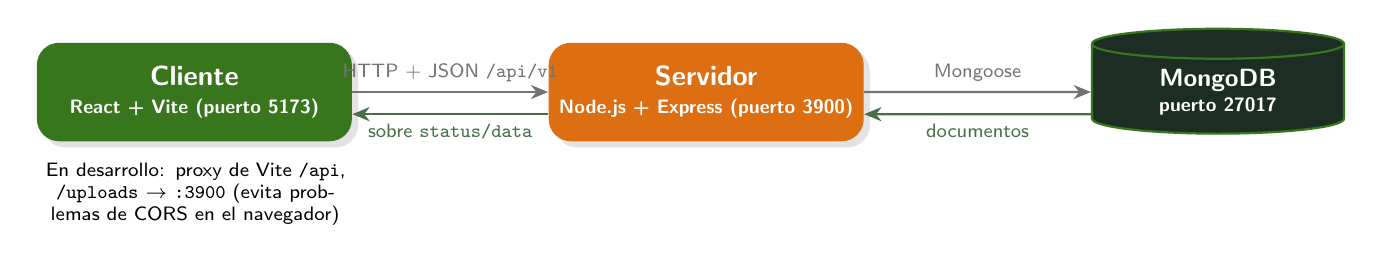
\begin{tikzpicture}
  \node[state,fill=mayorgreen,minimum width=4cm] (cli) at (0,0) {Cliente\\[-2pt]{\scriptsize React + Vite (puerto 5173)}};
  \node[state,fill=lyservice,minimum width=4cm] (api) at (6.5,0) {Servidor\\[-2pt]{\scriptsize Node.js + Express (puerto 3900)}};
  \node[cylinder,shape border rotate=90,aspect=0.22,fill=lydb,draw=mayorgreen,line width=0.8pt,text=white,
        font=\sffamily\bfseries\small,align=center,minimum width=3.2cm,minimum height=1.3cm] (db) at (13,0) {MongoDB\\[-2pt]{\scriptsize puerto 27017}};
  \draw[arr] (cli.east) -- node[above,font=\sffamily\scriptsize]{HTTP + JSON \code{/api/v1}} (api.west);
  \draw[arrg] ([yshift=-8pt]api.west) -- node[below,font=\sffamily\scriptsize]{sobre \code{status/data}} ([yshift=-8pt]cli.east);
  \draw[arr] (api.east) -- node[above,font=\sffamily\scriptsize]{Mongoose} (db.west);
  \draw[arrg] ([yshift=-8pt]db.west) -- node[below,font=\sffamily\scriptsize]{documentos} ([yshift=-8pt]api.east);
  \node[font=\sffamily\scriptsize,align=center,text width=4cm] at (0,-1.3) {En desarrollo: proxy de Vite \code{/api}, \code{/uploads} $\rightarrow$ \code{:3900} (evita problemas de CORS en el navegador)};
\end{tikzpicture}
\caption{Arquitectura general: cliente, servidor y base de datos.}
\end{figure}

\subsection{Diagrama de capas}

\begin{figure}[H]
\centering
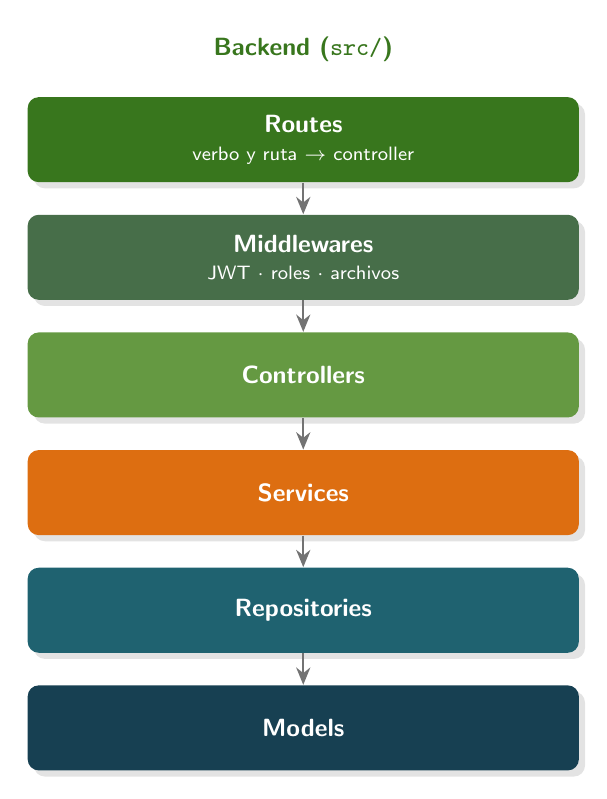
\begin{tikzpicture}[x=1cm,y=1cm]
  \node[layer,fill=lyroutes] (rt) at (0,0) {\textbf{Routes}\\[-1pt]{\scriptsize verbo y ruta $\rightarrow$ controller}};
  \node[layer,fill=lymiddle,below=0.4cm of rt] (mw) {\textbf{Middlewares}\\[-1pt]{\scriptsize JWT $\cdot$ roles $\cdot$ archivos}};
  \node[layer,fill=lycontrol,below=0.4cm of mw] (ct) {\textbf{Controllers}};
  \node[layer,fill=lyservice,below=0.4cm of ct] (sv) {\textbf{Services}};
  \node[layer,fill=lyrepo,below=0.4cm of sv] (rp) {\textbf{Repositories}};
  \node[layer,fill=lymodel,below=0.4cm of rp] (md) {\textbf{Models}};
  \foreach \a/\b in {rt/mw,mw/ct,ct/sv,sv/rp,rp/md}{\draw[arr] (\a) -- (\b);}
  \node[font=\sffamily\bfseries\small,color=mayorgreen] at ([yshift=0.6cm]rt.north) {Backend (\code{src/})};
\end{tikzpicture}\hspace{1.2cm}
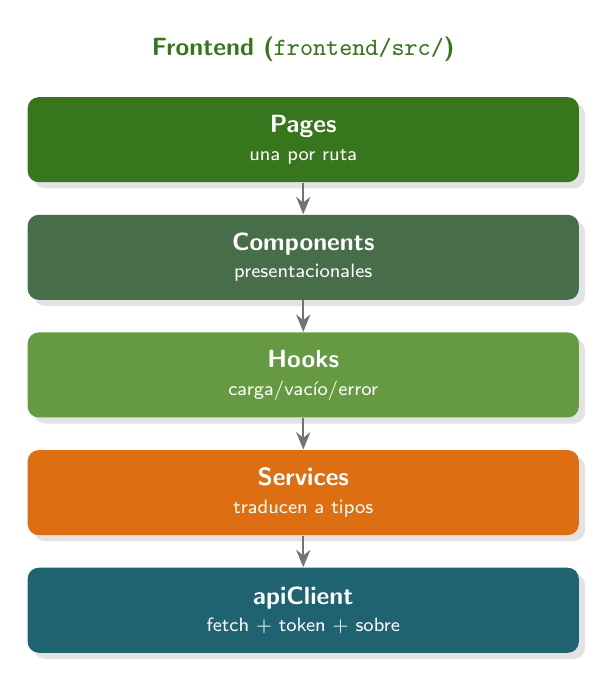
\begin{tikzpicture}[x=1cm,y=1cm]
  \node[layer,fill=lypage] (pg) at (0,0) {\textbf{Pages}\\[-1pt]{\scriptsize una por ruta}};
  \node[layer,fill=lycomp,below=0.4cm of pg] (cp) {\textbf{Components}\\[-1pt]{\scriptsize presentacionales}};
  \node[layer,fill=lyhook,below=0.4cm of cp] (hk) {\textbf{Hooks}\\[-1pt]{\scriptsize carga/vacío/error}};
  \node[layer,fill=lysvc,below=0.4cm of hk] (sc) {\textbf{Services}\\[-1pt]{\scriptsize traducen a tipos}};
  \node[layer,fill=lyapi,below=0.4cm of sc] (ap) {\textbf{apiClient}\\[-1pt]{\scriptsize fetch + token + sobre}};
  \foreach \a/\b in {pg/cp,cp/hk,hk/sc,sc/ap}{\draw[arr] (\a) -- (\b);}
  \node[font=\sffamily\bfseries\small,color=mayorgreen] at ([yshift=0.6cm]pg.north) {Frontend (\code{frontend/src/})};
\end{tikzpicture}
\caption{Capas del backend y del frontend, verificadas contra el árbol real del repositorio.}
\end{figure}

\begin{codebox}[language=tree,basicstyle=\ttfamily\fontsize{7.2}{8.8}\selectfont]{mayorgreen}{src/ (backend, 32 archivos .ts)}
routes/        user.ts, publication.ts, reservation.ts, notification.ts
middlewares/   auth.ts, roles.ts, upload.ts, errorHandler.ts
controllers/   user.ts, publication.ts, reservation.ts, notification.ts
services/      auth.service.ts, user.service.ts, publication.service.ts,
               reservation.service.ts, notification.service.ts, jwt.ts
repositories/  user.repository.ts, publication.repository.ts,
               reservation.repository.ts, notification.repository.ts
models/        user.ts, publication.ts, reservation.ts, notification.ts
types/         domain.ts, express.d.ts
utils/         AppError.ts, response.ts, serializePublication.ts, escapeRegex.ts
database/      connection.ts
\end{codebox}

\begin{codebox}[language=tree,basicstyle=\ttfamily\fontsize{7.2}{8.8}\selectfont]{mayorgreen}{frontend/src/ (62 archivos)}
pages/       LoginPage, RegisterPage, FeedPage, PublicationDetailPage,
             MyDonationsPage, CreatePublicationPage, AdminReviewPage,
             NotificationsPage, ProfilePage, NotFoundPage
components/  Header, Navbar, Layout, Loading, EmptyState, ErrorMessage,
             ProtectedRoute, RoleRoute, PublicationCard, AuthLayout,
             ChangePasswordForm
hooks/       useAuth, usePublications, usePublication, useReservations,
             useNotifications, useProfile, useProfilePublications,
             useSavedPublications, useSavedPublicationsList
services/    apiClient, auth, users, publications, reservations,
             notifications, savedPublications
context/     AuthContext/Provider, SavedPublicationsContext/Provider
\end{codebox}

\subsection{Recorrido de una petición de punta a punta}

Ejemplo: reservar una necesidad desde el detalle de una publicación.

\begin{figure}[H]
\centering
\resizebox{\linewidth}{!}{%

\begin{tikzpicture}
  \node[flow,fill=lypage] (n1) at (0,0) {Click\\"Reservar"};
  \node[flow,fill=lysvc,right=0.3cm of n1] (n2) {services/\\reservations.ts};
  \node[flow,fill=lyapi,right=0.3cm of n2] (n3) {apiClient\\+ token};
  \node[flow,fill=lyroutes,right=0.3cm of n3] (n4) {routes/\\reservation.ts};
  \node[flow,fill=lymiddle,right=0.3cm of n4] (n5) {auth\\+ roles};
  \node[flow,fill=lycontrol,right=0.3cm of n5] (n6) {Controller};
  \node[flow,fill=lyservice,right=0.3cm of n6] (n7) {Service};
  \node[flow,fill=lyrepo,right=0.3cm of n7] (n8) {Repository\\(atómico)};
  \node[flow,fill=mayordark,right=0.3cm of n8] (n9) {Respuesta\\201};
  \node[flow,fill=lypage,right=0.3cm of n9] (n10) {UI: estado\\"reservado"};
  \foreach \a/\b in {n1/n2,n2/n3,n3/n4,n4/n5,n5/n6,n6/n7,n7/n8,n8/n9,n9/n10}{\draw[arr] (\a) -- (\b);}
\end{tikzpicture}}
\caption{Recorrido completo de \code{POST /api/v1/reservations}, desde el clic hasta la pantalla.}
\end{figure}

{\tablestyle
\begin{longtable}{@{}>{\raggedright\arraybackslash}p{3.2cm}>{\raggedright\arraybackslash}p{9.7cm}@{}}
\caption{Detalle del recorrido de punta a punta}\\
\rowcolor{mayorgreen}\hc{Paso} & \hc{Qué ocurre}\\
\endfirsthead
\rowcolor{mayorgreen}\hc{Paso} & \hc{Qué ocurre}\\
\endhead
Componente & \code{PublicationDetailPage.handleReserve(itemId)} deshabilita el botón y llama al service.\\
Service (frontend) & \code{reservationsService.create(publicationId, itemId)} construye el cuerpo.\\
\code{apiClient} & Agrega \code{Authorization: Bearer <token>}, hace el \code{fetch}, interpreta el sobre de respuesta.\\
Proxy de Vite & En desarrollo, \code{/api} se reenvía a \code{http://localhost:3900} (sin esto, el navegador vería un origen distinto).\\
Routes (backend) & \code{auth} valida el JWT; \code{roles(["donante"])} exige ese rol; si pasa, llama al controller.\\
Controller & Valida que \code{publication\_id} e \code{item\_id} vengan en el cuerpo (400 si no).\\
Service (backend) & Pide la actualización atómica al repositorio de publicaciones.\\
Repository & \code{findOneAndUpdate} condicionado (\code{status:"aprobada"} y necesidad \code{"disponible"}); si no hay coincidencia, no se crea nada y el service responde 409.\\
Éxito & Se crea el documento de \code{Reservation}, se notifica al beneficiario y se responde \code{201} con el sobre estándar.\\
UI & El componente recibe la reserva, muestra el banner de éxito y recarga el detalle: la necesidad pasa a mostrarse como "Reservado".\\
\end{longtable}}

\subsection{Contrato de la API final}

La tabla completa de endpoints, con parámetros, cuerpos y códigos de error, es la de \ruta{docs/informe-Hito2.md} (sección 3), ya corregida para coincidir con el código real (24 endpoints, no 19 como se había estimado). Aquí solo se resume lo que cambió desde ese cierre:

{\tablestyle
\begin{longtable}{@{}>{\raggedright\arraybackslash}p{3.3cm}>{\raggedright\arraybackslash}p{9.6cm}@{}}
\caption{Cambios al contrato de la API desde el Hito 2}\\
\rowcolor{mayorgreen}\hc{Qué} & \hc{Detalle}\\
\endfirsthead
\rowcolor{mayorgreen}\hc{Qué} & \hc{Detalle}\\
\endhead
Recursos nuevos & \code{/users/saved-publications} (3 endpoints) y \code{/notifications} (2 endpoints); ambos compatibles (versión menor, misma ruta \code{/api/v1}).\\
Parámetro nuevo & \code{search} opcional en \code{GET /publications}, busca por texto de la historia, nombre de necesidad o nombre del autor.\\
Cambio de contraseña & \code{PATCH /users/update} acepta opcionalmente \code{current\_password} + \code{new\_password}, mismo endpoint, sin ruta nueva.\\
Corrección de bug & \code{GET /users/profile/:id} ignoraba el \code{:id} y siempre devolvía el perfil propio; ahora respeta el parámetro.\\
Corrección de bug & \code{DELETE /publications/\{id\}} no verificaba reservas activas; ahora responde \code{409} si hay alguna \code{reservado}.\\
Ruta eliminada & \code{GET /users/list/\{page\}} (paginación por path, duplicada e inconsistente con el resto de la API).\\
\end{longtable}}

\subsection{Modelo de datos final}

Sin cambios de fondo respecto del Hito 2 (enfoque mixto: necesidades embebidas, el resto referenciado). Se agregó \code{saved\_publications} (arreglo de \code{ObjectId}) al esquema de \code{User}, para sostener "Guardados". El diagrama entidad-relación completo y los campos de cada colección están en \ruta{docs/informe-Hito2.md} (sección 5.1), ya actualizados.

\subsection{Decisión de despliegue}
\label{sec:despliegue}

\pendiente{No hay contenedores implementados (ni \code{Dockerfile} ni \code{docker-compose.yml} en el repositorio). Falta decidir y documentar aquí la estrategia de despliegue, con una alternativa comparada y su desventaja asumida, antes de cerrar esta sección.}

% ------------------------------------------------------------------ 4. EVOLUCIÓN DE DECISIONES
\section{Evolución de decisiones y bitácora}
\label{sec:evolucion}

\subsection{Qué cambió desde el Hito 1}

Los cambios ya justificados en el Hito 2 (confirmación de entrega manual en vez de foto, capa de \code{repositories}, contrato \code{/api/v1}, reducción de alcance, plan de empresa y Ley 21.440 diferidos) se mantienen sin modificación y no se repiten aquí; ver la sección de cambios de \ruta{docs/informe-Hito2.md}. Lo que cambió \textbf{entre el cierre del Hito 2 y este informe} es lo siguiente:

{\tablestyle
\begin{longtable}{@{}>{\raggedright\arraybackslash}p{3.2cm}>{\raggedright\arraybackslash}p{5.2cm}>{\raggedright\arraybackslash}p{4.3cm}@{}}
\caption{Cambios entre el Hito 2 y este informe}\\
\rowcolor{mayorgreen}\hc{Qué cambió} & \hc{Motivo} & \hc{Impacto}\\
\endfirsthead
\rowcolor{mayorgreen}\hc{Qué cambió} & \hc{Motivo} & \hc{Impacto}\\
\endhead
Frontend construido completo & Objetivo explícito del Hito 3: flujo principal de punta a punta & Backend sin cambios de contrato en esta parte\\
Guardados y Notificaciones wireadas al frontend & Necesidades reales detectadas al construir las pantallas & 5 endpoints nuevos, compatibles\\
Búsqueda en el feed & El buscador del navbar era decorativo desde el mockup del Hito 1 & 1 parámetro opcional nuevo\\
\code{GET /users/profile/:id} corregido & Encontrado al redactar este informe: ignoraba el \code{:id} & Ahora cualquiera puede ver el perfil público de otro usuario, como pedía el diseño original\\
\code{DELETE /publications/\{id\}} corregido & Encontrado al redactar este informe: no chequeaba reservas activas & Ahora da \code{409} en vez de borrar con reservas en curso\\
\code{CORS\_ORIGIN} corregido & \code{app.use(cors())} ignoraba la variable de entorno & Ahora el origen es configurable de verdad\\
\code{db/init.ts} reescrito & El script original (\code{db/init.js}) estaba roto desde la migración a TypeScript; no había script \code{npm} que lo ejecutara & Ahora \code{npm run db:init} funciona y además crea datos de prueba (beneficiario, donante, publicación aprobada)\\
Documentación reconciliada & \ruta{docs/endpoints.md}, \ruta{informe-tecnico.md}, \ruta{modelo-datos.md} y \ruta{persistencia-credenciales.md} describían un contrato viejo (rutas \code{/auth/*} inexistentes, sin Notificaciones/Guardados) & Los cuatro documentos se actualizaron contra el código real\\
\end{longtable}}

\subsection{Bitácora de decisiones (resumen)}

Versión completa, con fecha y detalle de cada entrada, en \ruta{docs/bitacora.md}. Resumen de las decisiones más relevantes para la arquitectura final:

{\tablestyle
\begin{longtable}{@{}>{\raggedright\arraybackslash}p{3.4cm}>{\raggedright\arraybackslash}p{4.6cm}>{\raggedright\arraybackslash}p{4.7cm}@{}}
\caption{Bitácora de decisiones (resumen)}\\
\rowcolor{mayorgreen}\hc{Decisión} & \hc{Motivo} & \hc{Qué salió mal / cómo se resolvió}\\
\endfirsthead
\rowcolor{mayorgreen}\hc{Decisión} & \hc{Motivo} & \hc{Qué salió mal / cómo se resolvió}\\
\endhead
Usar el código real como fuente de verdad, no \code{CLAUDE.md} ni documentos previos & El backend tenía cambios sin documentar y los documentos estaban desactualizados & Se detectaron varias rutas inexistentes (\code{/auth/*}) antes de construir el frontend sobre ellas\\
Mass-assignment en \code{PATCH /users/update} & Se encontró que cualquier campo del cuerpo se guardaba sin filtrar & Cualquiera podía autoasignarse \code{role: "admin"}; se corrigió con lista blanca de campos\\
Avatar dejó de subirse tras el fix anterior & El whitelist de campos no incluía \code{image} (que viene de multer, no del usuario) & Se separó \code{updateAvatar} del flujo general de actualización\\
Guardados como referencias, no copias & Evitar duplicar datos de la publicación & \code{\$addToSet}/\code{\$pull} para que la operación sea idempotente\\
Búsqueda con texto de usuario en \code{\$regex} & Riesgo de inyección de regex / ReDoS & Se agregó \code{escapeRegex()} antes de construir el filtro\\
\code{GET /reservations} para el rol \code{admin} & Se detectó que ese rol cae en la misma rama que \code{donante} (filtra por \code{donor\_id}, casi siempre vacío) & Documentado como comportamiento real, no se cambió (no estaba pedido)\\
\end{longtable}}

% ------------------------------------------------------------------ 5. VALIDACIÓN, ERRORES Y ESTADOS
\section{Validación, errores y estados}

\subsection{Qué se valida y dónde}

{\tablestyle
\begin{longtable}{@{}>{\raggedright\arraybackslash}p{3.0cm}>{\raggedright\arraybackslash}p{5.0cm}>{\raggedright\arraybackslash}p{4.9cm}@{}}
\caption{Validación en cliente y en servidor}\\
\rowcolor{mayorgreen}\hc{Capa} & \hc{Qué valida} & \hc{Ejemplo}\\
\endfirsthead
\rowcolor{mayorgreen}\hc{Capa} & \hc{Qué valida} & \hc{Ejemplo}\\
\endhead
Cliente (formularios) & Campos obligatorios, largos máximos, formato de correo, al menos una necesidad al crear publicación & \code{maxLength} en inputs, validación antes de enviar\\
Cliente (\code{apiClient}) & Interpreta el sobre, traduce \code{401} a cierre de sesión & Redirección a \code{/login} con aviso\\
Servidor (controllers) & Presencia de campos obligatorios en el cuerpo & \code{AppError("VALIDATION\_ERROR", 400, ...)}\\
Servidor (services) & Reglas de negocio, propiedad del recurso, transiciones de estado & p. ej. solo el donante cancela su reserva\\
Servidor (errorHandler) & Traduce errores de Mongoose (\code{ValidationError}, \code{CastError}, código 11000) & 400 / 400 / 409\\
\end{longtable}}

El cliente \textbf{nunca} es la autoridad: toda regla validada en el frontend se vuelve a validar en el servidor.

\subsection{Código de error de la API → mensaje al usuario}

{\tablestyle
\begin{longtable}{@{}>{\raggedright\arraybackslash}p{3.4cm}>{\raggedright\arraybackslash}p{9.2cm}@{}}
\caption{Traducción de errores de la API a lenguaje de usuario}\\
\rowcolor{mayorgreen}\hc{Código de la API} & \hc{Mensaje al usuario}\\
\endfirsthead
\rowcolor{mayorgreen}\hc{Código de la API} & \hc{Mensaje al usuario}\\
\endhead
\code{VALIDATION\_ERROR} & "Revisa los campos marcados" (más el detalle por campo)\\
\code{UNAUTHENTICATED} / sesión expirada & "Tu sesión expiró. Inicia sesión de nuevo"\\
\code{FORBIDDEN} & "No tienes permiso para esta acción"\\
\code{NOT\_FOUND} & "Esto ya no está disponible"\\
\code{NEED\_NOT\_AVAILABLE} & "Otra persona reservó este ítem hace un momento. Elige otro"\\
Sin conexión con el servidor & "No pudimos conectar. Revisa tu conexión y reintenta"\\
\code{INTERNAL\_ERROR} & "Algo salió mal de nuestro lado. Intenta de nuevo"\\
\end{longtable}}

\subsection{Estados de carga, vacío y error}

Todas las pantallas que cargan datos (\code{FeedPage}, \code{PublicationDetailPage}, \code{MyDonationsPage}, \code{AdminReviewPage}, \code{NotificationsPage}, \code{ProfilePage}) implementan los tres estados mediante los componentes compartidos \code{Loading}, \code{EmptyState} y \code{ErrorMessage} (este último con botón de reintento). Ninguna pantalla puede quedar en blanco.

\pendiente{Agregar una captura de cada estado (carga/vacío/error) para al menos una pantalla, probada apagando el backend a propósito.}

% ------------------------------------------------------------------ 6. MANUAL
\section{Manual de uso e instalación}

Versión resumida; el manual completo está en \ruta{docs/manual.md} (Fase 1: creado junto con este esqueleto). El \code{README.md} de la raíz debe enlazarlo cuando el manual quede cerrado.

\subsection{Requisitos}
\begin{itemize}
\item Node.js (versión usada en desarrollo: \porcompletar{confirmar versión exacta con \texttt{node -v}}).
\item MongoDB corriendo en \code{localhost:27017} (se levanta a mano; no hay contenedor).
\item npm.
\end{itemize}

\subsection{Instalación}
\begin{enumerate}
\item Clonar el repositorio.
\item Backend: \code{npm install}, copiar \code{.env.example} a \code{.env}, \code{npm run db:init} (crea el admin y datos de prueba — \textbf{destructivo}, borra la base), \code{npm run dev}.
\item Frontend: \code{cd frontend}, \code{npm install}, copiar \code{.env.example} a \code{.env}, \code{npm run dev}.
\item Abrir \code{http://localhost:5173}.
\end{enumerate}

\pendiente{Esta instalación no se probó en un equipo limpio (sin Node/Mongo preinstalados ni dependencias ya descargadas). Antes de entregar, probarla de verdad en una máquina aparte o declarar explícitamente que no se probó.}

\subsection{Usuarios y datos de prueba}

{\tablestyle
\begin{longtable}{@{}>{\raggedright\arraybackslash}p{4.3cm}>{\raggedright\arraybackslash}p{2.6cm}>{\raggedright\arraybackslash}p{2.0cm}>{\raggedright\arraybackslash}p{3.6cm}@{}}
\caption{Cuentas de prueba creadas por \code{npm run db:init}}\\
\rowcolor{mayorgreen}\hc{Correo} & \hc{Contraseña} & \hc{Rol} & \hc{Para probar}\\
\endfirsthead
\rowcolor{mayorgreen}\hc{Correo} & \hc{Contraseña} & \hc{Rol} & \hc{Para probar}\\
\endhead
\code{admin@robin.com} & \code{admin123} & admin & Moderación de publicaciones\\
\code{beneficiario@robin.com} & \code{beneficiario123} & beneficiario & Crear/editar publicaciones; ya tiene una aprobada\\
\code{donante@robin.com} & \code{donante123} & donante & Reservar, cancelar, confirmar entrega\\
\end{longtable}}

Todas son cuentas ficticias, creadas solo para pruebas (consistente con la regla de no usar datos personales reales).

\subsection{Fallas frecuentes}

{\tablestyle
\begin{longtable}{@{}>{\raggedright\arraybackslash}p{4.2cm}>{\raggedright\arraybackslash}p{8.4cm}@{}}
\caption{Fallas encontradas durante el desarrollo y su solución}\\
\rowcolor{mayorgreen}\hc{Falla} & \hc{Solución}\\
\endfirsthead
\rowcolor{mayorgreen}\hc{Falla} & \hc{Solución}\\
\endhead
\code{ECONNREFUSED} al conectar a Mongo & MongoDB no está corriendo. Levantarlo antes de \code{npm run dev} (no se gestiona con un contenedor).\\
Puerto \code{3900} o \code{5173} ocupado & Otro proceso (otra instancia de \code{npm run dev}) ya lo está usando; identificarlo y detenerlo antes de levantar uno nuevo.\\
El frontend no ve al backend & El proxy de Vite apunta a \code{http://localhost:3900}; si el backend corre en otro puerto, hay que ajustar \code{vite.config.ts}.\\
\end{longtable}}

\subsection{Guía de uso por rol}

Ver la tabla de roles de la sección~2.3. El flujo paso a paso (sección~2.2) aplica directamente usando las cuentas de prueba de esta sección.

% ------------------------------------------------------------------ 7. LIMITACIONES DECLARADAS
\section{Limitaciones declaradas}
\label{sec:limitaciones}

\begin{itemize}
\item \textbf{Sin pruebas automatizadas:} ni backend ni frontend tienen un framework de testing configurado; toda la verificación fue manual.
\item \textbf{Token en \code{localStorage}:} vulnerable a XSS (declarado explícitamente, ver Anexo B). No hay refresco de token ni revocación del lado del servidor.
\item \textbf{Sin despliegue en contenedores:} no hay \code{Dockerfile} ni \code{docker-compose.yml}; la decisión de despliegue queda \porcompletar{pendiente (sección~\ref{sec:despliegue})}.
\item \textbf{Sin índices compuestos:} las colecciones \code{publications}, \code{reservations} y \code{notifications} solo tienen el índice \code{\_id} por defecto; las consultas por \code{status}, \code{donor\_id} o \code{user\_id} no tienen índice de soporte (sin impacto observable con el volumen actual de datos).
\item \textbf{\code{CORS\_ORIGIN} sin verificar en producción:} el código ya lee la variable, pero no se confirmó que el \code{.env} real tenga un valor restrictivo (una prueba con un origen arbitrario devolvió \code{Access-Control-Allow-Origin: *}).
\item \textbf{Plan de empresa / comisión de afiliado:} fuera de alcance técnico desde el Hito 2 (depende de una entidad donataria registrada bajo la Ley 21.440); no implementado.
\item \textbf{Confirmación de entrega:} la hace cualquiera de las dos partes por separado, sin evidencia fotográfica ni confirmación cruzada obligatoria.
\item \textbf{\code{GET /reservations} para el rol \code{admin}:} no tiene un caso especial; devuelve las reservas donde el admin sería "donante" (casi siempre vacío). No es un caso de uso real del producto, pero es un comportamiento no intuitivo del endpoint.
\item \textbf{Sin CI:} no hay integración continua configurada.
\end{itemize}

% ------------------------------------------------------------------ 8. CONCLUSIÓN
\section{Conclusión}

Este hito cerró la promesa planteada desde el Hito 1: una wishlist de bienes donde un beneficiario publica necesidades concretas, un administrador modera la publicación y un donante reserva y entrega directamente uno de los bienes. A diferencia de los informes anteriores, este describe un producto que se pudo usar de punta a punta, con el frontend real conectado al backend real, no una maqueta ni un contrato de API documentado pero sin probar contra una interfaz.

El resultado alcanzado coincidió con lo comprometido en el Hito 2 en lo esencial —arquitectura en capas, reserva atómica de necesidades, confirmación manual de entrega— y lo superó en algunos puntos que no estaban previstos: notificaciones consultables, publicaciones guardadas y búsqueda en el feed, surgidos de necesidades reales al construir la interfaz y no de un plan original. También se encontraron y corrigieron, durante la redacción de este mismo informe, tres errores de comportamiento del backend que habían pasado inadvertidos hasta entonces (sección~\ref{sec:evolucion}), lo que confirmó el valor de contrastar la documentación contra el código real antes de darla por cerrada, en vez de asumir que el código hacía lo que el documento decía.

Quedó fuera lo declarado en la sección~\ref{sec:limitaciones}: pruebas automatizadas, despliegue en contenedores, y lo que ya estaba fuera de alcance desde el Hito 2 por razones legales o de tiempo (comisión de afiliado, certificado de donación, plan de empresa). Si el proyecto continuara, el trabajo pendiente más concreto sería decidir e implementar una estrategia de despliegue, agregar al menos pruebas automatizadas para la reserva atómica —la regla de negocio más crítica del sistema— y cerrar las brechas de privacidad declaradas en el Anexo B.

% ------------------------------------------------------------------ 9. REFERENCIAS
\section{Referencias}

\begin{itemize}
\item Express. (s. f.-a). \textit{Error handling}. \href{https://expressjs.com/en/guide/error-handling.html}{https://expressjs.com/en/guide/error-handling.html}
\item Express. (s. f.-b). \textit{Express: Node.js web application framework}. \href{https://expressjs.com/}{https://expressjs.com/}
\item Express. (s. f.-c). \textit{Routing}. \href{https://expressjs.com/en/guide/routing.html}{https://expressjs.com/en/guide/routing.html}
\item Express. (s. f.-d). \textit{Using middleware}. \href{https://expressjs.com/en/guide/using-middleware.html}{https://expressjs.com/en/guide/using-middleware.html}
\item Fielding, R., Nottingham, M., \& Reschke, J. (2022). \textit{HTTP semantics} (RFC 9110). RFC Editor. \href{https://www.rfc-editor.org/info/rfc9110}{https://www.rfc-editor.org/info/rfc9110}
\item Jones, M., Bradley, J., \& Sakimura, N. (2015). \textit{JSON Web Token (JWT)} (RFC 7519). RFC Editor. \href{https://www.rfc-editor.org/info/rfc7519}{https://www.rfc-editor.org/info/rfc7519}
\item MongoDB. (s. f.). \textit{MongoDB manual}. \href{https://www.mongodb.com/docs/manual/}{https://www.mongodb.com/docs/manual/}
\item Mongoose. (s. f.). \textit{Schemas}. \href{https://mongoosejs.com/docs/guide.html}{https://mongoosejs.com/docs/guide.html}
\item React. (s. f.). \textit{React}. \href{https://react.dev/}{https://react.dev/}
\item React Router. (s. f.). \textit{React Router documentation}. \href{https://reactrouter.com/}{https://reactrouter.com/}
\item Vite. (s. f.). \textit{Vite}. \href{https://vite.dev/}{https://vite.dev/}
\item \porcompletar{Ley 21.719 y Ley 19.628 (Anexo B) — verificar texto vigente contra bcn.cl antes de citar artículos específicos.}
\end{itemize}

% ------------------------------------------------------------------ ANEXO A
\section{Anexo A — Uso de inteligencia artificial}

Declaración basada en lo efectivamente ocurrido en las sesiones de trabajo con Claude Code; \porcompletar{el equipo debe confirmar si se usó alguna otra herramienta de IA fuera de estas sesiones antes de considerar este anexo cerrado}.

\subsection{Herramientas y alcance}

{\tablestyle
\begin{longtable}{@{}>{\raggedright\arraybackslash}p{2.6cm}>{\raggedright\arraybackslash}p{3.3cm}>{\raggedright\arraybackslash}p{6.7cm}@{}}
\caption{Herramientas de IA usadas y alcance}\\
\rowcolor{mayorgreen}\hc{Herramienta} & \hc{Alcance} & \hc{Verificación}\\
\endfirsthead
\rowcolor{mayorgreen}\hc{Herramienta} & \hc{Alcance} & \hc{Verificación}\\
\endhead
Claude Code & Construcción del frontend completo; correcciones de backend; documentación (este informe, \ruta{docs/informe-Hito2.md} y los documentos previos) & Pruebas manuales con \code{curl} contra el backend real para cada endpoint tocado; uso real en navegador para cada pantalla; \code{grep} de separación de capas; recompilación del PDF para verificar que el LaTeX generado compila sin errores.\\
\end{longtable}}

\subsection{Qué se rechazó o corrigió de lo generado por IA}

\begin{itemize}
\item La primera versión de la tabla de "índices" en \ruta{persistencia-credenciales.md} describía índices compuestos que no existen en los esquemas reales; se verificó con \code{grep -i index src/models} (sin resultados) y se corrigió la documentación en vez de inventar que el índice existía.
\item El documento \ruta{informe-Hito2.md} describía la confirmación de entrega como "ambas partes deben confirmar"; el código real solo exige una de las dos partes. Se corrigió la documentación para que coincida con el código, no al revés.
\item Varias rutas documentadas en \ruta{endpoints.md} e \ruta{informe-tecnico.md} (p. ej. \code{/auth/register}) nunca existieron en el código; se detectó al revisar \code{src/routes/} directamente y se corrigieron.
\item Tres bugs reales de backend (\code{GET /users/profile/:id} ignorando el \code{:id}, \code{DELETE /publications/\{id\}} sin chequear reservas activas, \code{CORS\_ORIGIN} sin leerse) se encontraron al redactar esta documentación, se presentaron como opciones al equipo antes de corregirlos, y se corrigieron solo tras la aprobación explícita.
\end{itemize}

\subsection{Qué decidió el equipo, no la IA}

Cada vez que la IA encontró una diferencia entre lo documentado y el código, o una brecha de implementación, se le presentaron al equipo las alternativas (corregir el código, o documentar la brecha tal como está) antes de actuar; la decisión final, en todos los casos, fue del equipo:
\begin{itemize}
\item Corregir en el código, y no solo documentar, los cuatro errores de backend encontrados en esta revisión (\code{DELETE /publications/\{id\}} sin chequear reservas activas, \code{GET /users/profile/:id} ignorando el \code{:id}, la ruta duplicada \code{/users/list/\{page\}}, \code{CORS\_ORIGIN} sin leerse).
\item Documentar, en vez de implementar, la ausencia de índices compuestos en los esquemas: el equipo priorizó que la documentación dijera la verdad por sobre agregar código no pedido.
\item Agregar datos de prueba reproducibles (\code{beneficiario}, \code{donante}, una publicación aprobada) al script \code{db/init.ts}, en vez de dejar que el manual exigiera crear cuentas a mano.
\item Actualizar los documentos previos del Hito 2 (\ruta{endpoints.md}, \ruta{informe-tecnico.md}, \ruta{modelo-datos.md}, \ruta{persistencia-credenciales.md}) en vez de archivarlos o reemplazarlos.
\item Usar \ruta{docs/informe-Hito2.md} como plantilla de estilo y estructura para este informe.
\item El alcance de cada funcionalidad nueva del frontend (notificaciones, publicaciones guardadas, búsqueda) y su diseño visual específico (qué información mostrar, dónde ubicar cada botón) fueron pedidos explícitamente por el equipo, pantalla por pantalla, no propuestos por la IA.
\item Quitar la sub-sección "Lecciones aprendidas" de este informe fue una decisión explícita del equipo.
\end{itemize}

% ------------------------------------------------------------------ ANEXO B
\section{Anexo B — Análisis de datos personales}

\subsection{Inventario de datos que trata Robin}

{\tablestyle
\begin{longtable}{@{}>{\raggedright\arraybackslash}p{2.6cm}>{\raggedright\arraybackslash}p{4.5cm}>{\raggedright\arraybackslash}p{5.5cm}@{}}
\caption{Datos personales tratados por el sistema}\\
\rowcolor{mayorgreen}\hc{Dato} & \hc{Dónde vive} & \hc{Clasificación}\\
\endfirsthead
\rowcolor{mayorgreen}\hc{Dato} & \hc{Dónde vive} & \hc{Clasificación}\\
\endhead
Nombre, apellido, apodo & \code{users.name}, \code{surname}, \code{nick} & Identificación básica\\
Correo & \code{users.email} & Identificación, usado como credencial de inicio de sesión\\
Contraseña (hash bcrypt) & \code{users.password} & Credencial; nunca se devuelve en ninguna respuesta\\
Dirección, teléfono & \code{users.address}, \code{phone} & Datos de contacto; opcionales\\
Rol & \code{users.role} & Determina permisos\\
Necesidades declaradas & {\scriptsize\code{publications.necesidades[].name}} & Puede revelar situación de vulnerabilidad del beneficiario (ej. qué le falta a su familia)\\
Historial de reservas & \code{reservations} & Vincula donante y beneficiario\\
Notificaciones & \code{notifications.message} & Puede contener referencias indirectas a lo anterior\\
\end{longtable}}

Las necesidades declaradas por un beneficiario pueden calificar como datos de una persona en situación de vulnerabilidad; el sistema no las trata con ninguna protección adicional respecto del resto de los datos.

\subsection{Finalidad y base de licitud}

Todo el tratamiento tiene como finalidad única la operación del servicio (ejecución del contrato implícito al registrarse): conectar beneficiarios con donantes. No hay tratamiento con fines publicitarios, de perfilamiento ni de venta a terceros. La base de licitud es el consentimiento al registrarse (acepta implícitamente que sus datos de perfil y sus necesidades sean visibles para otros usuarios autenticados) \porcompletar{confirmar si existe o debería existir una aceptación explícita de términos al registrarse; hoy no la hay}.

\subsection{Principios}

\begin{itemize}
\item \textbf{Minimización:} no se pide RUT, fecha de nacimiento ni datos bancarios (no hay manejo de dinero).
\item \textbf{Proporcionalidad:} dirección y teléfono son opcionales en el registro.
\item \textbf{Seguridad:} contraseñas hasheadas con bcrypt, JWT con expiración, \code{.env} fuera del repositorio.
\item \textbf{Transparencia:} \porcompletar{hoy no hay una política de privacidad visible en la interfaz; declarar como brecha.}
\end{itemize}

\subsection{Medidas aplicadas}

\begin{itemize}
\item Hash de contraseñas con bcrypt; nunca se devuelven en ninguna respuesta (\code{.select("-password")} redundante en el repositorio).
\item JWT con expiración configurable, payload mínimo (\code{id}, \code{role}), sin datos personales dentro del token.
\item Credenciales de base de datos y JWT fuera del repositorio (\code{.env}, con \code{.env.example} sin valores reales).
\item Control de acceso por rol en middlewares, y de propiedad del recurso en los services.
\item Datos ficticios en todas las cuentas de prueba del repositorio.
\end{itemize}

\subsection{Derechos de los titulares}

El producto \textbf{no} implementa hoy ningún mecanismo de acceso, rectificación o eliminación de la cuenta más allá de \code{PATCH /users/update} (edición parcial del propio perfil). No existe un endpoint para que un usuario elimine su cuenta ni para que exporte sus datos. Se declara como brecha, no como funcionalidad pendiente de descubrir en la defensa.

\subsection{Riesgos y brechas pendientes}

\begin{itemize}
\item Token en \code{localStorage}, vulnerable a robo por XSS (ver Limitaciones).
\item Sin política de retención ni borrado automático de notificaciones o reservas antiguas.
\item Sin registro (\textit{logging}) de accesos a datos sensibles.
\item Sin consentimiento explícito al registrarse (checkbox de términos, por ejemplo).
\item \porcompletar{Verificar contra el texto vigente de la Ley 21.719 (y Ley 19.628 hasta su entrada en vigencia plena) qué obligaciones concretas aplican y si alguna de ellas es exigible para un proyecto académico; no citar artículos sin verificar contra bcn.cl.}
\end{itemize}

% ------------------------------------------------------------------ ANEXO C
\section{Anexo C — Bitácora, capturas y colección de pruebas}

\begin{itemize}
\item \textbf{Bitácora completa:} \ruta{docs/bitacora.md}.
\item \textbf{Capturas de pantalla:} \porcompletar{no existen todavía en el repositorio; agregar antes de cerrar el informe.}
\item \textbf{Colección de pruebas (Postman u otra):} \porcompletar{no existe todavía; se usó \texttt{curl} manual durante el desarrollo. Decidir si se exporta una colección formal o se documenta como no entregada.}
\end{itemize}

\subsection*{Glosario}

{\tablestyle
\begin{longtable}{@{}>{\raggedright\arraybackslash}p{3.0cm}>{\raggedright\arraybackslash}p{9.8cm}@{}}
\caption{Glosario de términos de dominio y técnicos}\\
\rowcolor{mayorgreen}\hc{Término} & \hc{Significado}\\
\endfirsthead
\rowcolor{mayorgreen}\hc{Término} & \hc{Significado}\\
\endhead
Necesidad & Ítem concreto (un bien, no dinero) que un beneficiario pide dentro de una publicación; subdocumento embebido con su propio estado (\code{disponible}, \code{reservado}, \code{entregado}).\\
Publicación & Historia de un beneficiario junto con su lista de necesidades; nace \code{pendiente} y solo es visible en el feed cuando un admin la aprueba.\\
Moderación & Revisión de una publicación por el rol \code{admin}, que la cambia a \code{aprobada} o \code{rechazada} antes de que sea pública.\\
Reserva & Vínculo entre un donante y una necesidad concreta; su estado (\code{reservado}, \code{entregado}, \code{cancelada}) es independiente del estado de la necesidad, aunque cambian juntos.\\
Reserva atómica & Actualización de la necesidad resuelta en una sola operación de base de datos (\code{findOneAndUpdate} condicionado), para que dos donantes no puedan reservar el mismo ítem al mismo tiempo.\\
Confirmación manual & La entrega se marca como completada por una de las dos partes (donante o beneficiario) desde la plataforma, sin evidencia fotográfica.\\
Sobre de respuesta & Estructura fija de toda respuesta de la API: \code{\{status, statusCode, data, meta?\}} en éxito, \code{\{status, statusCode, error\}} en error.\\
\code{AppError} & Clase de error que usan los \code{services} para señalar una regla de negocio incumplida; el \code{errorHandler} la traduce al sobre de error final.\\
Guardados & Lista personal de publicaciones que un usuario marcó para revisar después, sin que eso reserve ninguna necesidad.\\
Capa & Grupo de archivos con una única responsabilidad (\code{routes}, \code{controllers}, \code{services}, \code{repositories}, \code{models} en el backend; \code{pages}, \code{hooks}, \code{services} en el frontend), que solo puede llamar a la capa inmediatamente inferior.\\
\end{longtable}}

% ------------------------------------------------------------------ VERIFICACIÓN DE CAPAS (referencia interna)
\section*{Verificación de capas}
\label{sec:verificacion}
{\small
\begin{verbatim}
grep -rnE "mongoose|models/|repositories/" src/controllers   -> vacío
grep -rnE "req\.|res\.|mongoose" src/services                -> vacío
grep -rn "fetch(" frontend/src/pages frontend/src/components -> vacío
\end{verbatim}
}

\end{document}
